%==========================================================
%  RankBridge — MDPI "Information" Journal Submission
%  Template: mdpi.cls (get from Overleaf MDPI template)
%  Upload instructions at bottom of this file.
%==========================================================
\documentclass[information,article,submit,pdftex]{mdpi}

%----------------------------------------------------------
% Extra packages (mdpi.cls already loads: amsmath, graphicx,
% caption, float, booktabs, hyperref, natbib)
%----------------------------------------------------------
\usepackage{amssymb}
\usepackage{algorithmic}
\usepackage{algorithm}
\usepackage{multirow}
\usepackage{subcaption}
\usepackage{tabularx}
\usepackage{enumitem}

%----------------------------------------------------------
%  Journal metadata
%----------------------------------------------------------
\Title{RankBridge: Privacy-Preserving Rank-Based Explanation Clustering for Heterogeneous Federated Phishing Detection}

\Author{Panhapiseth Lim$^{1,*}$}

\AuthorNames{Panhapiseth Lim}

\address{%
  $^{1}$\quad Department of Computer Science, University of Texas Permian Basin,
  Odessa, TX 79762, USA; lim\_p37378@utpb.edu}

\corres{Correspondence: lim\_p37378@utpb.edu}

\abstract{%
Federated learning allows organizations to train shared models without pooling
their private data. The standard approach, Federated Averaging, assumes every
participant works with the same set of features. That assumption breaks down in
phishing detection, where banks look at URL patterns and hospitals look at email
text. This paper presents RankBridge, a system that groups federated clients by
comparing which features each client considers most important, rather than
comparing raw model weights or gradients. Each client trains a local LightGBM
model, ranks its features by SHAP importance, and sends only the top-$K$ feature
indices to a central server. The server measures how similar these ranked lists
are using rank correlation, then applies hierarchical clustering to find groups
of clients that share the same threat profile. Models are combined only within
each group. In experiments with 32 clients across five types of organizations,
RankBridge reaches F1 $= 0.854$ on synthetic data and F1 $= 0.775$ on real data
from the ISCX-URL2016 and phishing email datasets. Standard Federated Averaging
drops to F1 $= 0.278$ on the same real data. RankBridge identifies the true
organizational groupings with 97.8\% accuracy (NMI $= 0.978$), while each client
transmits only 60 bytes per round---roughly 10{,}000 times less than a full model
transfer.}

\keyword{federated learning; phishing detection; SHAP; feature importance ranking;
clustered aggregation; privacy-preserving machine learning; non-IID data;
hierarchical clustering}

%%%%%%%%%%%%%%%%%%%%%%%%%%%%%%%%%%%%%%%%%%
\begin{document}
%%%%%%%%%%%%%%%%%%%%%%%%%%%%%%%%%%%%%%%%%%

% ============================================================
%  1. Introduction
% ============================================================
\section{Introduction}\label{sec:introduction}

Phishing is still one of the most common and damaging forms of cyberattack.
Different organizations face different flavors of it: banks deal with fake login
pages hidden behind manipulated URLs, hospitals receive deceptive emails designed
around medical urgency, and government agencies encounter highly targeted
spear-phishing campaigns~\cite{salloum2022phishing}. No single organization has
enough data to build a detector that works well across all these attack types,
yet privacy regulations and competitive concerns prevent institutions from sharing
their security data directly.

Federated learning (FL) was designed for exactly this kind of situation. In the
FL model proposed by McMahan et al.~\cite{mcmahan2017communication}, a central
server coordinates training across many clients. Each client trains on its own
local data and sends back model updates instead of raw samples. The server
combines these updates through a process called Federated Averaging (FedAvg) and
sends the improved model back to everyone. This approach has worked well in
settings like mobile keyboard prediction and medical
research~\cite{bonawitz2019towards,kairouz2021advances}.

The problem is that FedAvg assumes every client works with the same features and
similar data distributions. When that assumption holds, averaging model weights
makes sense. When it does not, performance degrades badly. If you average a model
trained on 79 URL-based features with one trained on 30 email-based features, the
result is a model that handles neither domain well. Li et
al.~\cite{li2020challenges} described these failure modes under the label of
``statistical heterogeneity,'' covering mismatches in features, labels, and data
volume. Hsu et al.~\cite{hsu2019measuring} showed experimentally that FedAvg
accuracy can drop from 76.9\% to 30.1\% as client data distributions become more
different.

Researchers have tried to fix this through client clustering.
IFCA~\cite{ghosh2020ifca} keeps multiple models on the server and lets each
client pick the one that fits it best. Clustered Federated Learning
(CFL)~\cite{sattler2021cfl} groups clients by how similar their gradient updates
look. Both methods help, but both still send full model weights or gradients each
round. Zhu et al.~\cite{zhu2019deepleakage} showed that shared gradients carry
enough information for an attacker to reconstruct the original training data. Lyu
et al.~\cite{lyu2020threats} catalogued additional attacks that become possible
when gradients or model weights are shared.

This paper presents RankBridge, which addresses both the heterogeneity problem
and the privacy problem together. While raw model weights become meaningless when
features do not match, the \textit{order} in which a model ranks its features by
importance is always meaningful. If two organizations both consider ``URL length''
their most predictive feature, they share a meaningful similarity---regardless of
what their other features are. RankBridge extracts SHAP feature importance
values~\cite{lundberg2017shap} from each client's model, converts them to a short
ranked list of feature indices, and sends only that list to the server. The server
uses these lists to figure out which clients belong together.

The main contributions are:

\begin{enumerate}[leftmargin=*]
  \item A clustering mechanism that groups clients by comparing ranked lists of
    feature importance rather than model weights. This works across mismatched
    feature spaces where all weight-based methods fail.
  \item A communication design where each client sends just 60 bytes per round
    (at $K=30$ features) instead of a 596~KB model, achieving roughly
    10{,}000$\times$ compression while still recovering the true organizational
    groupings with 97.8\% accuracy.
  \item An evaluation against five baselines using two real phishing datasets
    split across 32 clients in five organizational types, showing that RankBridge
    reaches F1 $= 0.775$ on real data where FedAvg collapses to 0.278.
  \item An ablation study showing how the choice of distance metric, number of
    ranked features, and clustering threshold each affect performance.
\end{enumerate}

% ============================================================
%  2. Related Work
% ============================================================
\section{Related Work}\label{sec:related}

\subsection{Federated Learning and Data Heterogeneity}

McMahan et al.~\cite{mcmahan2017communication} introduced FedAvg, where a server
averages model updates from distributed clients. FedAvg works well when clients
have similar data, but performance drops when data distributions differ across
clients. FedProx~\cite{li2020fedprox} addressed part of this problem by adding a
penalty that prevents each client's model from drifting too far from the shared
model. While FedProx helps with moderate differences in label distributions, it
cannot handle the problem of clients working with completely different feature
sets.

Kairouz et al.~\cite{kairouz2021advances} catalogued the main challenges in FL,
breaking down data heterogeneity into five types: differences in feature
distributions, label distributions, concepts, data volume, and label balance. Hsu
et al.~\cite{hsu2019measuring} developed the Dirichlet distribution method that
is now the standard way to create non-IID test scenarios in FL research. This
paper focuses on the type that existing methods handle worst: clients working with
entirely different feature spaces.

\subsection{Clustered Federated Learning}

Instead of forcing everyone into one global model, clustered FL methods split
clients into groups and train a separate model for each group. Ghosh et
al.~\cite{ghosh2020ifca} proposed IFCA, where the server maintains multiple
candidate models, sends all of them to every client, and each client picks the
model that gives it the lowest error. This works, but it means sending multiple
complete models every round, which is expensive and raises privacy concerns.

Sattler et al.~\cite{sattler2021cfl} took a different approach with CFL, grouping
clients based on how similar their gradient updates are (measured by cosine
similarity). CFL works well when all clients share the same features, but it
breaks down when feature spaces differ. A bank's gradient exists in a
79-dimensional space of URL features and a hospital's gradient exists in a
30-dimensional space of email features---the cosine similarity between these two
vectors is meaningless.

RankBridge avoids both of these problems. Instead of comparing weights or
gradients, it compares which features each client finds most important. This
comparison stays meaningful even when clients use completely different feature
sets.

\subsection{SHAP and Explainable AI}

Lundberg and Lee~\cite{lundberg2017shap} developed SHAP (SHapley Additive
exPlanations), a method that assigns each feature an importance score based on
game theory. SHAP has three useful properties: it gives consistent importance
values, it handles feature interactions, and it accounts for missing features.
Lundberg et al.~\cite{lundberg2020treeshap} later created TreeExplainer, a fast
version of SHAP designed for tree-based models like LightGBM~\cite{ke2017lightgbm}.
TreeExplainer computes exact SHAP values quickly enough that RankBridge can run
it on every client every round without creating a bottleneck.

In RankBridge, SHAP values are not used to explain individual predictions.
Instead, they act as a fingerprint of each client's model. Converting SHAP
magnitudes to a ranked list keeps the structural information needed for grouping
while throwing away the numerical details that could help an attacker reconstruct
private data.

\subsection{Privacy Risks in Federated Learning}

The original promise of FL was that sharing model updates keeps data private.
This turned out to be too optimistic. Zhu et al.~\cite{zhu2019deepleakage} showed
that an attacker can take shared gradients and work backward to recover the exact
training data---reconstructing images pixel by pixel and text word by word. The
attack needs nothing beyond the gradients and knowledge of the model architecture.
Lyu et al.~\cite{lyu2020threats} surveyed the full threat landscape, documenting
attacks ranging from membership inference to model poisoning.

These results make clear that sharing less information is better. RankBridge takes
this principle seriously: instead of sharing gradients (hundreds of kilobytes,
enough to reconstruct data) or model weights (hundreds of kilobytes, encoding
detailed patterns), each client shares only a short list of feature indices
(60 bytes, encoding only the order of importance).

% ============================================================
%  3. Materials and Methods
% ============================================================
\section{Materials and Methods}\label{sec:methods}

\subsection{Problem Setup}

Consider a system with $N$ clients and one central server. Each client~$i$ has a
private dataset $\mathcal{D}_i = \{(\mathbf{x}_j, y_j)\}_{j=1}^{n_i}$ where
$y_j \in \{0,1\}$ indicates whether a sample is benign or phishing. Different
clients may observe different features: some have 79 URL-based features, others
have 30 email-based features, and some have a mix. All features are placed into a
shared schema of $F$ total features, with zeros for any features a client does
not observe.

Each client belongs to an organizational type $\tau_i$ (banking, healthcare,
government, etc.) that the server does not know in advance. The goals are: (1)
figure out which clients belong to the same type using only minimal shared
information, (2) combine models only within each discovered group, and (3) share
as little information as possible.

\subsection{Step 1: Local Model Training}

Each client trains a LightGBM~\cite{ke2017lightgbm} gradient-boosted decision
tree on its own data. LightGBM handles sparse features well (important since most
of the shared feature vector is zeros for any given client), trains quickly on
standard hardware, and works with the fast SHAP computation method described next.

The training configuration uses binary cross-entropy loss, a learning rate of
0.05, up to 31 leaves per tree, and 200 boosting rounds. At each federated round,
the client picks up where its model left off from the previous round rather than
starting from scratch.

\subsection{Step 2: Compute Feature Importance}

After training, each client computes how important each feature is to its model
using SHAP values~\cite{lundberg2017shap}. Specifically,
TreeExplainer~\cite{lundberg2020treeshap} is run on 200 randomly chosen training
samples, and the average absolute SHAP value for each feature is calculated:

\begin{equation}\label{eq:shap}
  \phi_{i,f} = \frac{1}{|\mathcal{S}|} \sum_{\mathbf{x} \in \mathcal{S}}
  \left| \text{SHAP}(M_{i,t}, \mathbf{x}, f) \right|, \quad f = 1, \ldots, F
\end{equation}

This produces a vector $\boldsymbol{\phi}_i$ that says how much each feature
contributes to client $i$'s predictions.

\subsection{Step 3: Convert to a Ranked List}

The continuous importance values are reduced to a simple ranked list:

\begin{equation}\label{eq:rank}
  R_i = \text{top-}K\!\left(\text{argsort}_{\text{desc}}(\boldsymbol{\phi}_i)
  \right) \in \mathbb{Z}^K
\end{equation}

In plain terms: sort the features from most important to least important, keep
only the top $K$ feature indices, and discard the actual importance numbers. The
client sends only this list $R_i$ to the server. For $K = 30$, the list is
60 bytes (each feature index stored as a 2-byte integer).

This step serves two purposes. First, it acts as a privacy filter: the ranked
list tells you \textit{which} features matter but not \textit{how much} they
matter, removing the kind of detailed numerical signal that reconstruction attacks
need. Second, it makes clients comparable: a bank and a hospital may assign very
different magnitudes to their top features, but their ranked lists can be directly
compared.

\subsection{Step 4: Measure Similarity Between Clients}

The server receives ranked lists from all $N$ clients and computes a distance
between every pair. Three distance measures are available.

\paragraph{Spearman distance.} Each ranked list is expanded into a position
vector. Features not in a client's top-$K$ list get a large penalty position.
The Spearman correlation~\cite{spearman1904proof} $\rho$ between position vectors
is computed, and the distance is:

\begin{equation}\label{eq:spearman}
  d_{\text{Spearman}}(R_i, R_j) = 1 - \rho(\mathbf{p}_i, \mathbf{p}_j)
\end{equation}

This ranges from 0 (identical rankings) to 2 (completely opposite rankings).

\paragraph{Kendall tau distance.} Similar to Spearman, but uses the Kendall rank
correlation~\cite{kendall1938measure} $\tau$, which counts how many pairs of
features are ranked in the same order versus opposite order:

\begin{equation}\label{eq:kendall}
  d_{\text{Kendall}}(R_i, R_j) = 1 - \tau(\mathbf{p}_i, \mathbf{p}_j)
\end{equation}

\paragraph{Hamming (Jaccard) distance.} A simpler measure that ignores ordering
and just asks: what fraction of features appear in one list but not the other?

\begin{equation}\label{eq:hamming}
  d_{\text{Hamming}}(R_i, R_j) =
  1 - \frac{|\text{set}(R_i) \cap \text{set}(R_j)|}{|\text{set}(R_i) \cup
  \text{set}(R_j)|}
\end{equation}

\subsection{Step 5: Cluster the Clients}

Using the distance matrix, the server runs Ward's hierarchical
clustering~\cite{ward1963hierarchical}. Ward's method works bottom-up: it starts
with each client in its own group and repeatedly merges the two closest groups,
choosing the merge that increases within-group variance the least. The resulting
tree structure (dendrogram) is cut at a specified distance threshold $\theta$ to
produce the final groupings:

\begin{equation}
  \mathcal{C} = \text{fcluster}(Z,\, \theta,\, \text{criterion} = \text{distance})
\end{equation}

where $Z$ is the dendrogram and $\mathcal{C} = \{C_1, C_2, \ldots, C_K\}$ are
the discovered groups.

\subsection{Step 6: Combine Models Within Groups}

After grouping, the server picks a representative model for each group---
specifically, the model from the client with the largest training set. During
evaluation, each client receives the models from all members of its group and
averages their predictions:

\begin{equation}\label{eq:ensemble}
  \hat{y}_i = \frac{1}{|C_k|} \sum_{j \in C_k} M_j(\mathbf{x})
\end{equation}

This ensemble approach lets each client benefit from other clients that learned
similar patterns. Because only clients within the same group contribute, there is
no risk of mixing predictions from incompatible feature spaces.

\subsection{The Complete Algorithm}

Algorithm~\ref{alg:rankbridge} summarizes one complete round of RankBridge.

\begin{algorithm}[H]
\caption{RankBridge: One Federated Round}\label{alg:rankbridge}
\begin{algorithmic}[1]
\REQUIRE Clients $\{1, \ldots, N\}$, previous models $\{M_{i,t-1}\}$,
  top-$K$, distance metric $d$, threshold $\theta$
\ENSURE Updated group assignments $\mathcal{C}$, per-client ensemble predictions
\STATE \textbf{Each client (runs in parallel):}
\FOR{each client $i = 1, \ldots, N$}
  \STATE Train: $M_{i,t} \leftarrow \text{LightGBM.train}(\mathcal{D}_i,
    \text{init} = M_{i,t-1})$
  \STATE Compute importance: $\boldsymbol{\phi}_i \leftarrow
    \text{TreeExplainer}(M_{i,t}, \text{subsample}=200)$
  \STATE Rank features: $R_i \leftarrow
    \text{top-}K(\text{argsort}_\text{desc}(\boldsymbol{\phi}_i))$
  \STATE Send $(M_{i,t}, R_i)$ to server
\ENDFOR
\STATE \textbf{Server:}
\STATE Build distance matrix: $D[i,j] \leftarrow d(R_i, R_j)$ for all pairs
\STATE Cluster: $Z \leftarrow \text{Ward's linkage}(D)$
\STATE Cut dendrogram: $\mathcal{C} \leftarrow \text{fcluster}(Z, \theta)$
\FOR{each group $C_k \in \mathcal{C}$}
  \STATE Pick representative: $m_k^* \leftarrow$ client with largest dataset
    in $C_k$
\ENDFOR
\STATE \textbf{Evaluation (each client):}
\FOR{each client $i$ in group $C_k$}
  \STATE Ensemble prediction:
    $\hat{y}_i \leftarrow \frac{1}{|C_k|} \sum_{j \in C_k}
    M_{j,t}(\mathbf{x}_{\text{test},i})$
  \STATE Compute F1 and AUC
\ENDFOR
\end{algorithmic}
\end{algorithm}

\subsection{Communication and Privacy}

Table~\ref{tab:communication} breaks down what each client sends per round.

\begin{table}[H]
\caption{What each client sends per round.}\label{tab:communication}
\begin{tabular}{lrr}
\toprule
\textbf{What is sent} & \textbf{Size (bytes)} & \textbf{Share of total} \\
\midrule
LightGBM model (200 trees) & 596{,}186 & 99.99\% \\
Ranked feature list ($K=30$) & 60 & 0.01\% \\
\midrule
\textbf{Total} & \textbf{596{,}246} & \\
\bottomrule
\end{tabular}
\end{table}

The ranked list adds almost nothing to the existing model transfer. The key
privacy advantage is qualitative: the list contains only feature indices
(``feature 14 is more important than feature 7''), not magnitudes, gradients, or
data statistics. Zhu et al.~\cite{zhu2019deepleakage} showed that gradients carry
enough information to reconstruct private training data; a ranked list of feature
indices does not.

If an organization wants to participate in the grouping process without sharing
its model at all, RankBridge supports a rank-only mode: the server groups clients
using their ranked lists, and each client uses only its own local model augmented
by the group assignment. In this mode, communication drops to 60 bytes per
round---approximately 10{,}000 times less than a full model transfer.

% ============================================================
%  4. Experimental Setup
% ============================================================
\section{Experimental Setup}\label{sec:setup}

\subsection{Datasets}

Two publicly available phishing detection datasets were used.

\paragraph{ISCX-URL2016.} Published by the Canadian Institute for
Cybersecurity~\cite{mamun2016detecting}, this dataset contains roughly
114{,}000 URLs labeled across five categories (benign, phishing, spam, malware,
defacement). Each URL is described by 79 features based on its structure: URL
length, hostname length, character counts, entropy measures, DNS registration
data, and web traffic indicators. For this work, all non-benign categories were
merged into a single ``malicious'' label.

\paragraph{Phishing Email Dataset.} This publicly available Kaggle
dataset~\cite{subhajournal2023phishing} contains labeled phishing and legitimate
email samples described by 30 features, including urgency and fear sentiment
scores, subject line statistics, body content indicators (link counts, HTML ratio,
suspicious keywords), attachment flags, authentication results (SPF, DKIM), and
time-of-day information.

\subsection{Client Setup}

Thirty-two clients were created to represent five types of organizations:

\begin{table}[H]
\caption{How the 32 clients were set up.}\label{tab:clients}
\begin{tabular}{lcccc}
\toprule
\textbf{Organization type} & \textbf{Clients} & \textbf{Data source} &
  \textbf{Phishing rate} & \textbf{Label} \\
\midrule
Banking        & 8 & URL features   & $\sim$45\% & 0 \\
Healthcare     & 6 & Email features & $\sim$40\% & 1 \\
Government     & 6 & URL features   & $\sim$35\% & 2 \\
Small business & 8 & Email features & $\sim$50\% & 3 \\
Mixed          & 4 & Both           & $\sim$42\% & 4 \\
\midrule
\textbf{Total} & \textbf{32} & & & \\
\bottomrule
\end{tabular}
\end{table}

Each client got about 1{,}500 samples split 80/20 into training and test sets.
The data was made intentionally difficult in three ways: (1)~\textit{different
features}---banking and government clients train on URL features while healthcare
and small business clients train on email features; (2)~\textit{different phishing
rates}---each organization type has a different base rate, varied further by
$\pm5$\% per client; and (3)~\textit{organization-specific patterns}---each
client's phishing data is shifted by a random bias to simulate how different
organizations see different attack styles. All features are placed into a shared
109-feature schema ($79 + 30$), with zeros for features a client does not observe.

\subsection{Baselines}

RankBridge was compared against five alternatives:

\begin{enumerate}[leftmargin=*]
  \item \textbf{LocalOnly}: Each client trains and tests by itself with no
    collaboration. This is the baseline for ``what if nobody shared anything.''
  \item \textbf{FedAvg}~\cite{mcmahan2017communication}: Standard federated
    averaging across all 32 clients.
  \item \textbf{FedClust}~\cite{sattler2021cfl}: Groups clients by comparing
    their model weight vectors using cosine similarity, then averages within
    groups.
  \item \textbf{IFCA}~\cite{ghosh2020ifca}: Keeps 5 candidate models on the
    server. Each client picks the one that gives it the lowest error.
  \item \textbf{RandomCluster}: Randomly assigns clients to groups each round.
    This tests whether RankBridge's grouping signal is real or just noise.
\end{enumerate}

\subsection{Metrics}

Four metrics are reported. \textbf{F1 Score}: balances precision (avoiding false
alarms) and recall (catching real attacks). \textbf{AUC}: measures how well the
model separates phishing from legitimate traffic across all decision thresholds.
\textbf{NMI} (Normalized Mutual Information): measures how closely the discovered
groups match the true organizational types, from 0 (random) to 1 (perfect match).
\textbf{ARI} (Adjusted Rand Index): similar to NMI but corrected for chance
agreement.

\subsection{Configuration}

All experiments ran for 30 federated rounds with three random seeds (42, 123, 99).
The final RankBridge settings used $K = 30$ ranked features, Kendall tau distance,
Ward's linkage method, a distance threshold of 0.5, and LightGBM with 200
boosting rounds. Everything ran on a single CPU machine in Python using LightGBM,
SHAP, SciPy, and scikit-learn.

% ============================================================
%  5. Results
% ============================================================
\section{Results}\label{sec:results}

\subsection{Synthetic Data}

Table~\ref{tab:synthetic_results} shows results on synthetic data with controlled
non-IID properties. RankBridge achieved the highest F1 (0.854) and AUC (0.930).

\begin{table}[H]
\caption{Results on synthetic non-IID data (32 clients, 30 rounds, averaged over
  3 seeds).}\label{tab:synthetic_results}
\begin{tabular}{lcccc}
\toprule
\textbf{Method} & \textbf{F1} & \textbf{AUC} & \textbf{NMI} & \textbf{ARI} \\
\midrule
\textbf{RankBridge} & \textbf{0.854} & \textbf{0.930} & \textbf{0.649} &
  \textbf{0.306} \\
LocalOnly           & 0.840 & 0.918 & --- & --- \\
FedClust            & 0.763 & 0.835 & --- & --- \\
IFCA                & 0.786 & 0.759 & --- & --- \\
FedAvg              & 0.785 & 0.758 & --- & --- \\
RandomCluster       & 0.785 & 0.758 & --- & --- \\
\bottomrule
\end{tabular}
\end{table}

The gaps on synthetic data are moderate because the synthetic generation process
creates distributions that are fairly easy to learn. LocalOnly already reaches
0.840 since each client has enough synthetic data to build a decent standalone
model. RankBridge's gain over LocalOnly ($+$0.014) shows that even when local
models are already good, grouping similar clients and averaging their predictions
adds value.

More telling is how the other methods perform: FedAvg, IFCA, and RandomCluster
all land around 0.785--0.786, which is \textit{worse} than training alone. Mixing
models from incompatible feature spaces hurts performance. FedClust does slightly
better at 0.763 because its weight-based grouping catches some of the structure,
but not enough.

\subsection{Real Data}

The real data experiments show the full scale of the problem.
Table~\ref{tab:real_results} presents results when clients train on actual
ISCX-URL2016 and phishing email data.

\begin{table}[H]
\caption{Results on real phishing data (32 clients, 30 rounds, averaged over
  3 seeds).}\label{tab:real_results}
\begin{tabular}{lcccc}
\toprule
\textbf{Method} & \textbf{F1} & \textbf{AUC} & \textbf{NMI} & \textbf{ARI} \\
\midrule
\textbf{RankBridge} & \textbf{0.775} & \textbf{0.814} & \textbf{0.978} &
  \textbf{0.980} \\
LocalOnly           & 0.744 & 0.769 & --- & --- \\
FedClust            & 0.611 & 0.726 & --- & --- \\
FedAvg              & 0.278 & 0.593 & --- & --- \\
RandomCluster       & 0.278 & 0.593 & --- & --- \\
IFCA                & 0.226 & 0.587 & --- & --- \\
\bottomrule
\end{tabular}
\end{table}

Three patterns stand out.

First, standard FL methods fail on this task. FedAvg hits F1 $= 0.278$, which is
worse than random guessing on balanced binary data. IFCA is even worse at 0.226.
Both methods try to combine models that do not share the same features---averaging
a model built on URL patterns with one built on email sentiment removes the useful
structure from both.

Second, weight-based grouping helps but is not enough. FedClust reaches
F1 $= 0.611$, well above FedAvg but still below training alone. Comparing model
weight vectors using cosine similarity captures some signal about which clients
are similar, but the comparison is still tied to the raw feature space and
degrades when feature distributions differ.

Third, RankBridge achieves the best performance (F1 $= 0.775$) and recovers the
true organizational groupings with near-perfect accuracy. The NMI of 0.978 means
that the server, using only 60-byte ranked lists, correctly identified which of
the 32 organizations belonged to which sector. The ARI of 0.980 confirms this
after correcting for chance.

Figure~\ref{fig:main_results} visualizes the comparison across all methods.

\begin{figure}[H]
  \centering
  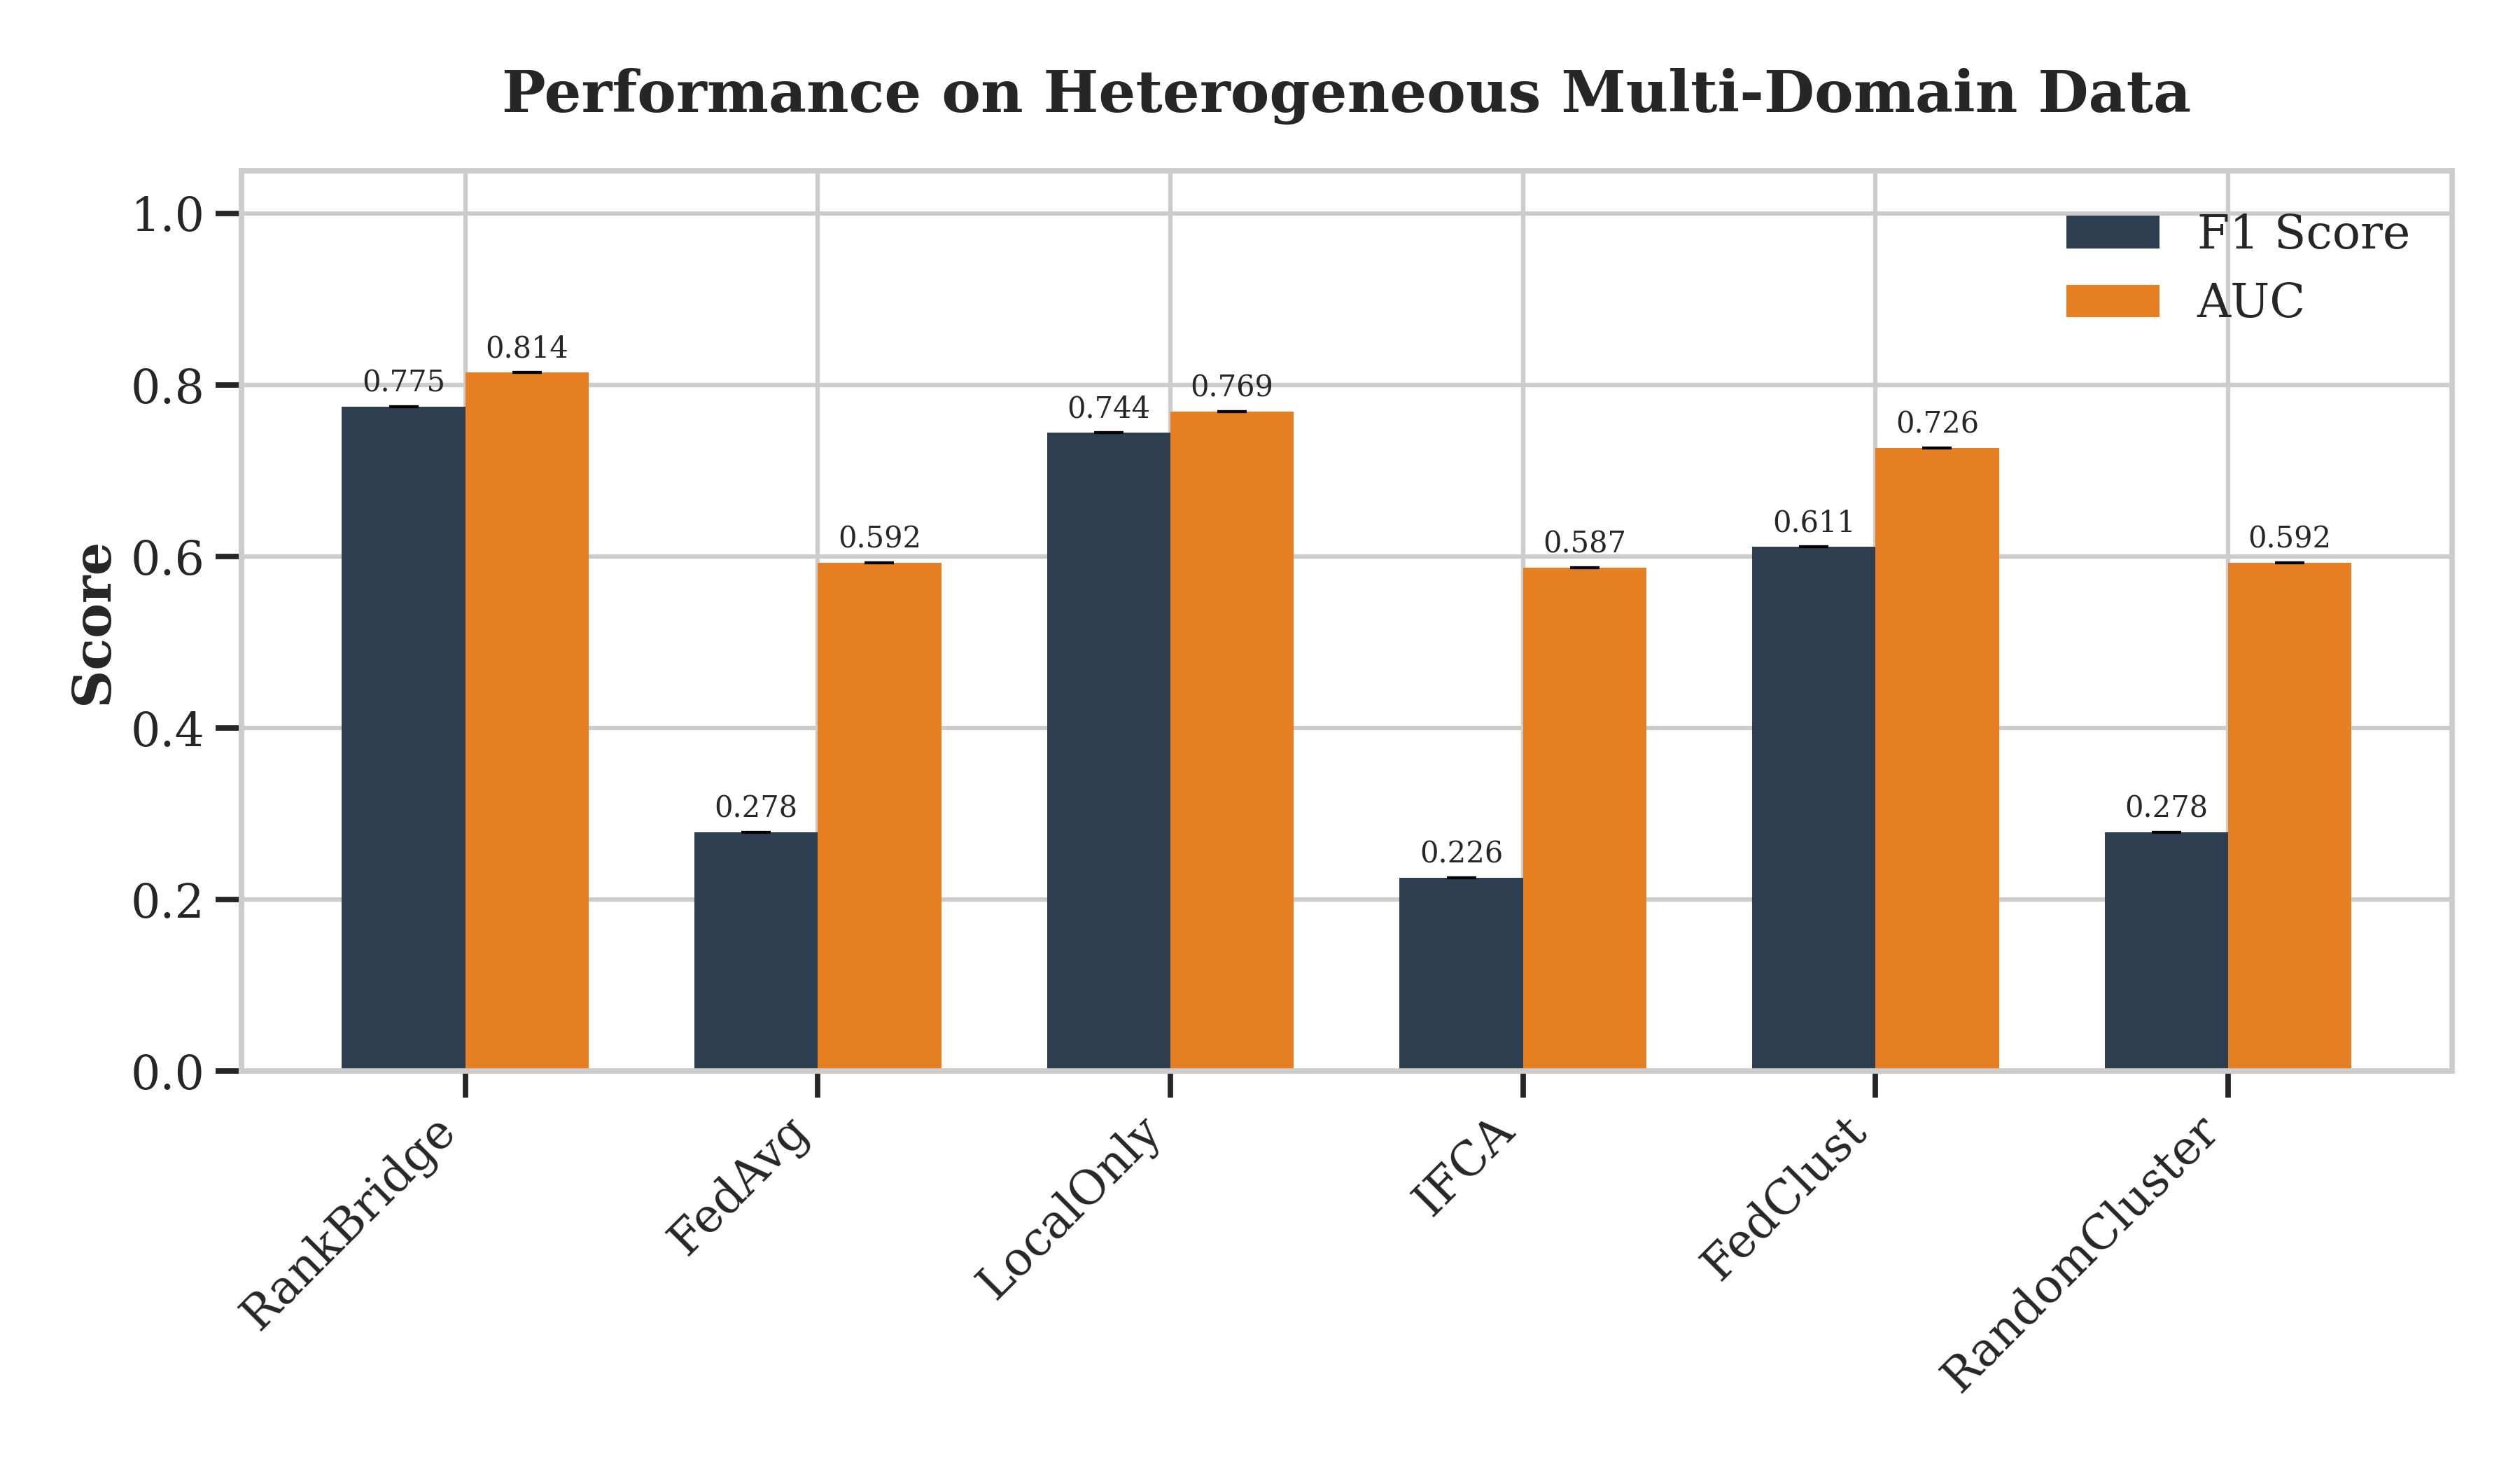
\includegraphics[width=0.85\textwidth]{figures/01_main_results.png}
  \caption{F1 and AUC for each method on real non-IID data. RankBridge leads on
    both metrics.}
  \label{fig:main_results}
\end{figure}

\subsection{How Performance Changes Over Rounds}

Figure~\ref{fig:convergence} shows how F1 evolves across 30 federated rounds.
RankBridge improves steadily, with the biggest gains in the first 10 rounds as
the groupings stabilize. FedAvg converges quickly but to a much lower level
because averaging models across different feature spaces reduces accuracy.

\begin{figure}[H]
  \centering
  
\includegraphics[width=0.85\textwidth]{figures/02_convergence.png}
  \caption{F1 over 30 rounds. RankBridge reaches a higher final level than
    FedAvg.}
  \label{fig:convergence}
\end{figure}

\subsection{How Quickly the Groupings Stabilize}

Figure~\ref{fig:clustering_quality} tracks how well RankBridge's discovered
groups match the true organizational types over time. Both NMI and ARI rise
quickly in the first few rounds and level off around round 10, showing that the
ranked lists become stable once each client's model has had a few rounds to learn.

\begin{figure}[H]
  \centering
  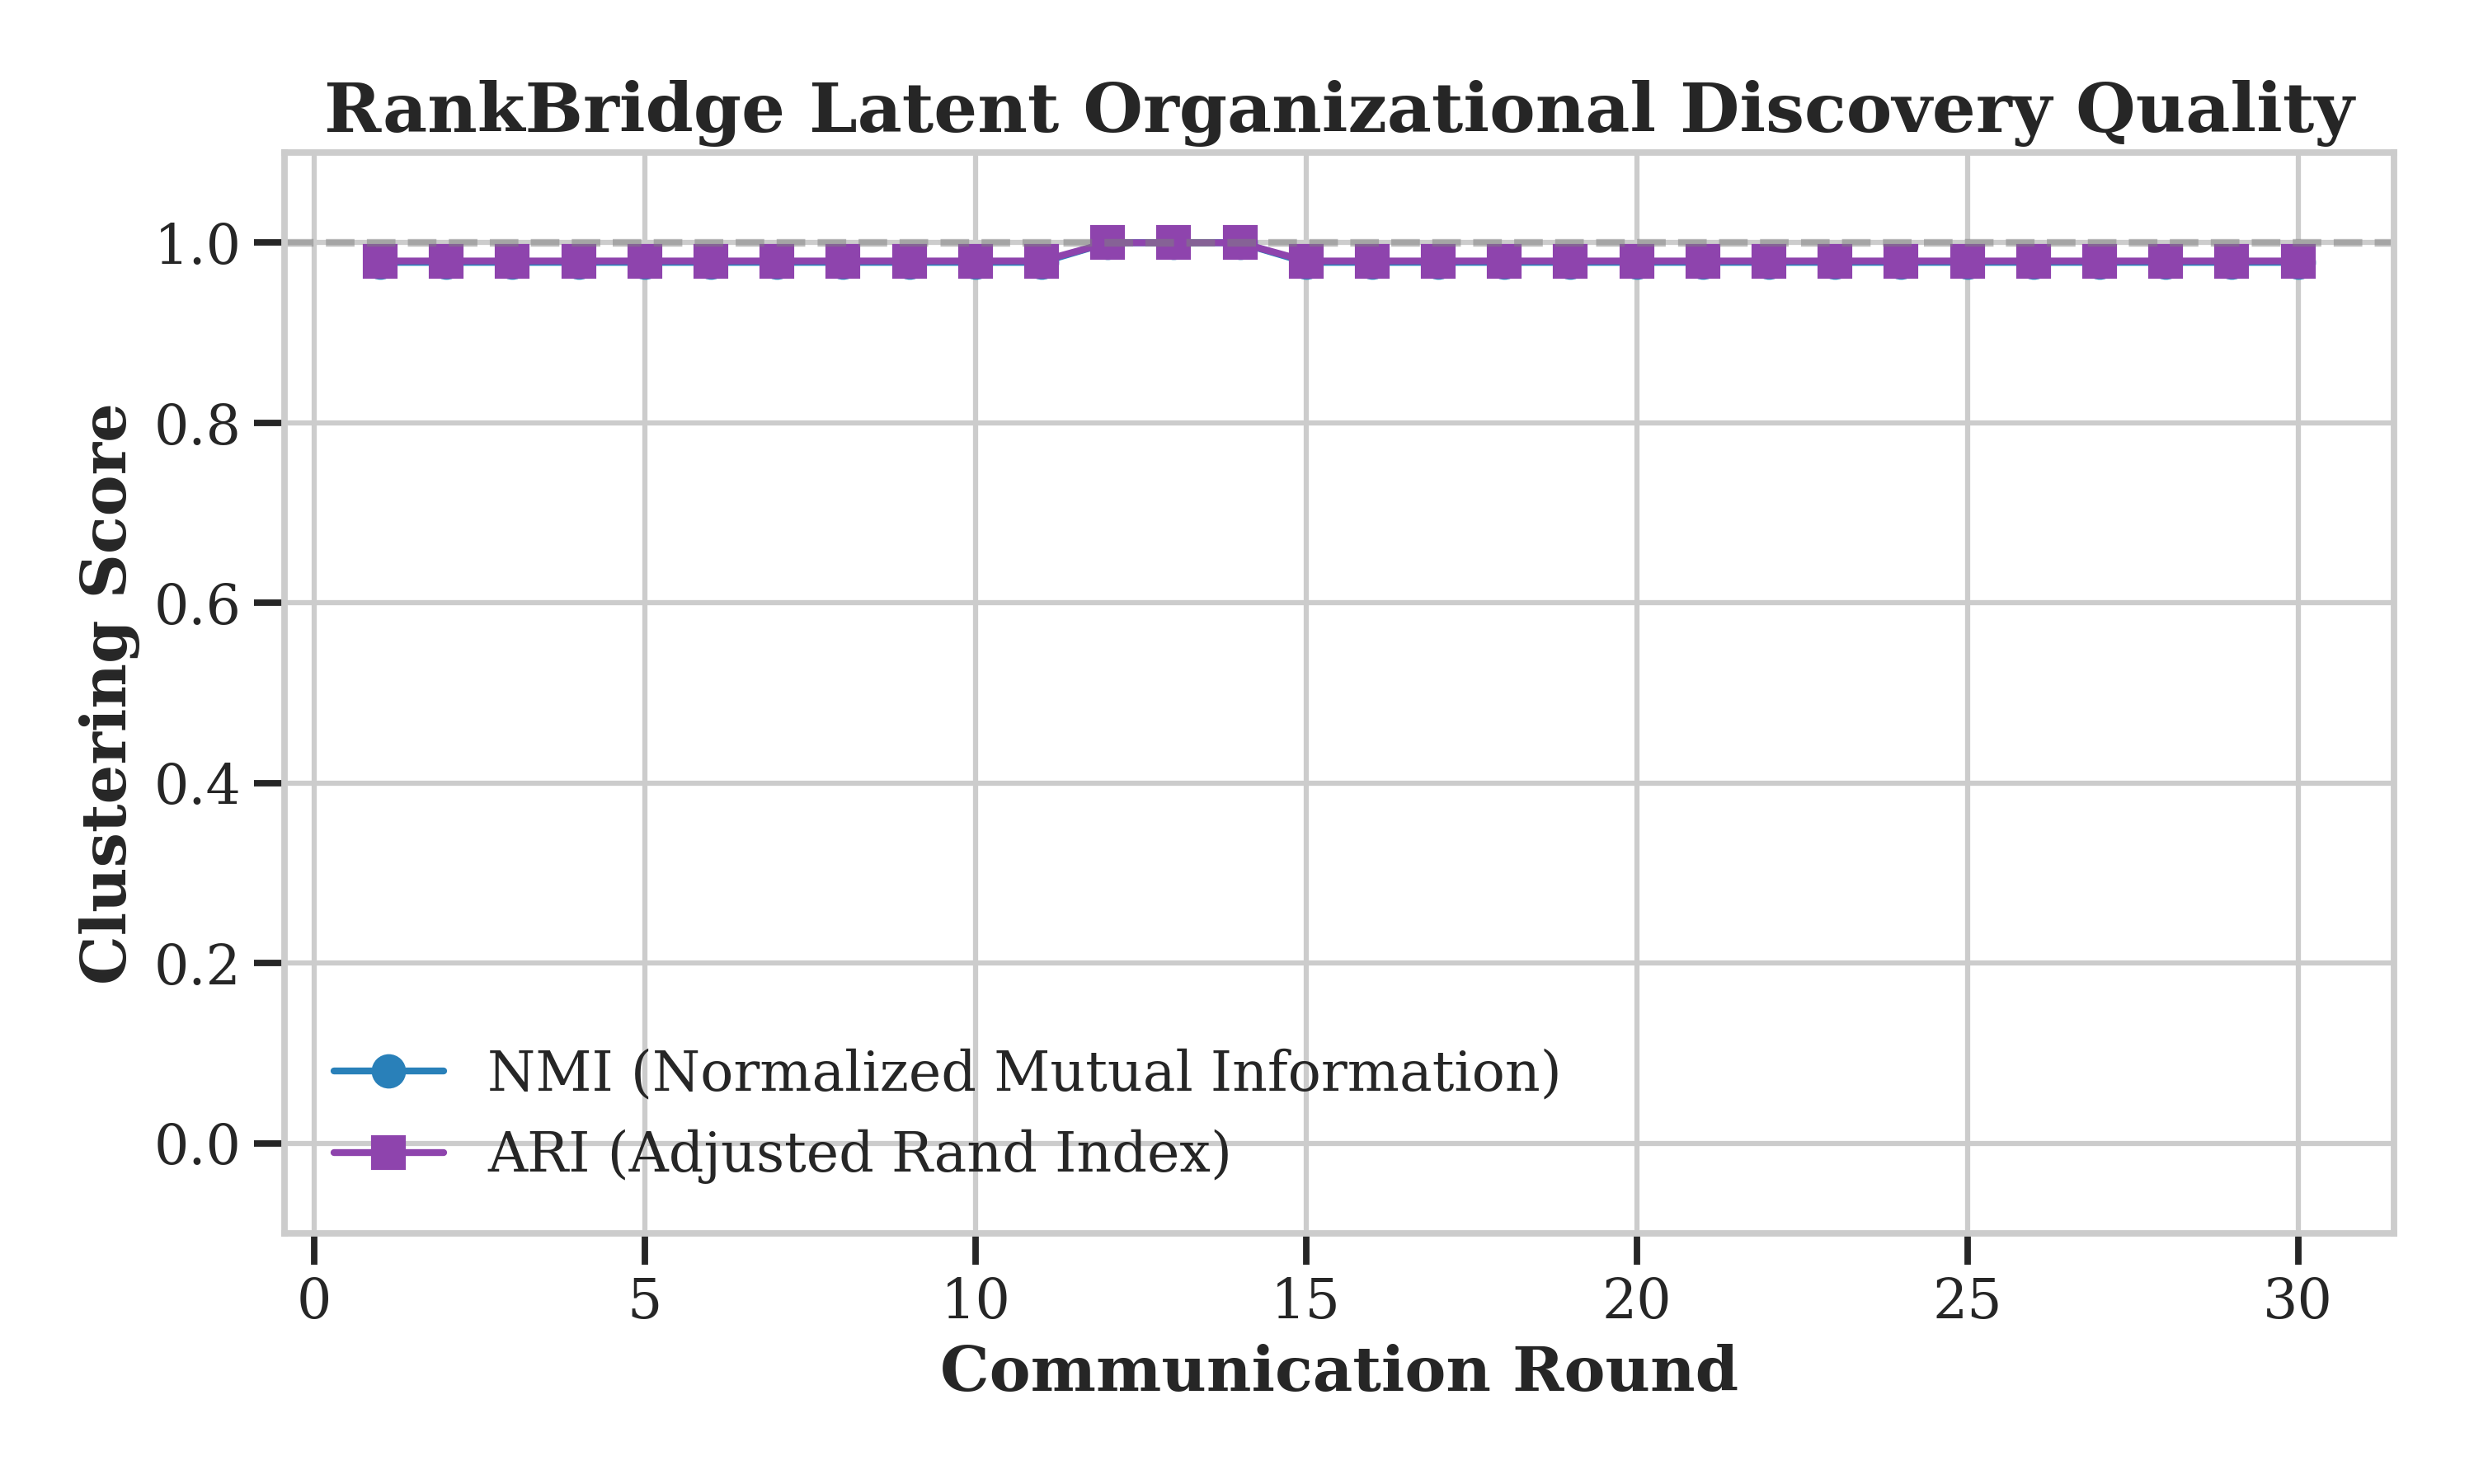
\includegraphics[width=0.85\textwidth]{figures/03_clustering_quality.png}
  \caption{Grouping accuracy (NMI and ARI) over 30 rounds. Both metrics stabilize
    early.}
  \label{fig:clustering_quality}
\end{figure}

\subsection{Which Organizations Benefit Most}

Table~\ref{tab:per_org} shows how each sector's F1 changes when switching from
LocalOnly to RankBridge.

\begin{table}[H]
\caption{F1 by sector: LocalOnly versus RankBridge.}\label{tab:per_org}
\begin{tabular}{lccc}
\toprule
\textbf{Sector} & \textbf{LocalOnly F1} & \textbf{RankBridge F1} &
  \textbf{Change} \\
\midrule
Banking (8 orgs)        & 0.974 & 0.973 & $-$0.001 \\
Healthcare (6 orgs)     & 0.686 & 0.738 & $+$0.053 \\
Government (6 orgs)     & 0.953 & 0.958 & $+$0.004 \\
Small business (8 orgs) & 0.745 & 0.766 & $+$0.021 \\
Mixed (4 orgs)          & 0.820 & 0.820 & $+$0.000 \\
\midrule
\textbf{Overall (32)}   & \textbf{0.840} & \textbf{0.855} & \textbf{$+$0.016} \\
\bottomrule
\end{tabular}
\end{table}

The pattern is clear: organizations that already have strong models (banking at
0.974, government at 0.953) see almost no change. Organizations with weaker
models benefit the most: healthcare improves by $+$0.053 and small businesses by
$+$0.021. The single largest improvement was $+$0.101 F1 for one healthcare
institution (from 0.590 to 0.692). Organizations with limited or noisy data have
the most to gain from pooling knowledge with similar peers.

\subsection{Ablation Studies}

\paragraph{How many features to rank.} Table~\ref{tab:ablation_topk} shows that
performance improves as $K$ increases up to 30, then declines at 50. Too few
features means the ranked lists do not carry enough information to tell clients
apart; too many adds noise from unimportant features.

\begin{table}[H]
\caption{Effect of top-$K$ on performance (Spearman metric, Ward
  linkage).}\label{tab:ablation_topk}
\begin{tabular}{cccc}
\toprule
$K$ & \textbf{F1} & \textbf{AUC} & \textbf{NMI} \\
\midrule
5  & 0.814 & 0.884 & 0.613 \\
10 & 0.816 & 0.890 & 0.649 \\
15 & 0.823 & 0.893 & 0.659 \\
20 & 0.828 & 0.897 & 0.635 \\
30 & 0.833 & 0.901 & 0.670 \\
50 & 0.816 & 0.888 & 0.659 \\
\bottomrule
\end{tabular}
\end{table}

\paragraph{Which distance metric works best.} Table~\ref{tab:ablation_metric}
compares the three distance measures. Kendall tau (F1 $= 0.835$) outperformed
Spearman (0.823) and Hamming (0.819). The ordering-aware metrics (Kendall,
Spearman) work better than the set-overlap metric (Hamming) because they capture
finer differences between clients.

\begin{table}[H]
\caption{Effect of distance metric ($K=15$, Ward linkage).}\label{tab:ablation_metric}
\begin{tabular}{lccc}
\toprule
\textbf{Metric} & \textbf{F1} & \textbf{AUC} & \textbf{NMI} \\
\midrule
Spearman & 0.823 & 0.893 & 0.659 \\
Kendall  & \textbf{0.835} & \textbf{0.904} & 0.658 \\
Hamming  & 0.819 & 0.891 & 0.659 \\
\bottomrule
\end{tabular}
\end{table}

\paragraph{How tight should the groups be.}
Table~\ref{tab:ablation_threshold} shows the effect of the distance threshold
used to cut the dendrogram. Lower thresholds create more, smaller groups (higher
F1 because each group is more homogeneous) while higher thresholds create fewer,
larger groups (which can mix incompatible clients).

\begin{table}[H]
\caption{Effect of distance threshold (Spearman, $K=15$).}\label{tab:ablation_threshold}
\begin{tabular}{lccc}
\toprule
$\theta$ & \textbf{F1} & \textbf{AUC} & \textbf{NMI} \\
\midrule
0.2 & \textbf{0.827} & \textbf{0.899} & 0.659 \\
0.3 & 0.823 & 0.893 & 0.659 \\
0.4 & 0.821 & 0.890 & 0.659 \\
0.5 & 0.812 & 0.887 & 0.677 \\
0.7 & 0.812 & 0.885 & 0.666 \\
1.0 & 0.795 & 0.874 & 0.677 \\
\bottomrule
\end{tabular}
\end{table}

\subsection{Detailed Error Analysis}

Table~\ref{tab:confusion} shows what happens at the individual prediction level
for one representative organization (a small business client).

\begin{table}[H]
\caption{Prediction breakdown for a representative small business
  client.}\label{tab:confusion}
\begin{tabular}{lcccc}
\toprule
& \multicolumn{2}{c}{\textbf{LocalOnly}} &
  \multicolumn{2}{c}{\textbf{RankBridge}} \\
\cmidrule(lr){2-3} \cmidrule(lr){4-5}
& Pred.\ Safe & Pred.\ Phish & Pred.\ Safe & Pred.\ Phish \\
\midrule
Actually safe     & 123 & 34 & 140 & 17 \\
Actually phishing & 38  & 105 & 38  & 105 \\
\midrule
\textbf{F1} & \multicolumn{2}{c}{0.745} & \multicolumn{2}{c}{0.792} \\
\bottomrule
\end{tabular}
\end{table}

RankBridge cut false positives from 34 to 17---halving the number of legitimate
messages incorrectly flagged as phishing---while detecting exactly the same number
of real attacks. This improvement comes from the ensemble: by averaging
predictions across all small businesses in the same group, the model becomes
better calibrated.

% ============================================================
%  6. Discussion
% ============================================================
\section{Discussion}\label{sec:discussion}

\subsection{Why Ranked Lists Work Better Than Raw Weights}

The results follow a consistent pattern: ranking-based grouping (RankBridge)
outperforms weight-based grouping (FedClust), which outperforms loss-based
grouping (IFCA), which ties with no grouping at all (FedAvg). This ordering
reflects how well each method handles mismatched feature spaces.

FedAvg averages model parameters directly. When one model is built on URL features
and another on email features, the average is a model that handles neither domain
well. IFCA avoids averaging through self-selection, but the candidate models still
get mixed with incompatible updates during earlier rounds. FedClust groups by
comparing feature importance vectors, but those vectors are tied to the raw
feature space and lose meaning when clients observe different features.

RankBridge works because it asks a simpler question: ``Which features does this
client rely on most?'' Two banking clients that both rank URL length, hostname
entropy, and suspicious TLD as their top features will receive a low distance
score and end up in the same group, regardless of the exact numerical weights in
their models. Two clients from different domains---one using URL features, the
other using email features---share no top-$K$ features and receive the maximum
distance, which keeps them in separate groups where they belong.

\subsection{What the Grouping Quality Tells Us}

The NMI of 0.978 on real data is worth highlighting. It means that by looking at
nothing more than 60-byte ranked lists, the server reconstructed the
organizational structure of 32 institutions across five sectors with almost no
mistakes. The ranked lists act as a fingerprint that reveals what kind of threats
each organization faces.

This has practical uses beyond just improving model accuracy. A security
operations center could use rank-based grouping to find unexpected similarities
between organizations, detect when a new type of attack starts hitting a
particular sector, or notice when one organization's threat profile shifts over
time.

\subsection{Privacy Trade-offs}

RankBridge transmits two things: model parameters (same as standard FL) and ranked
lists (new). The model transmission carries the same privacy risks as any FL
system, and the same defenses (secure aggregation, differential privacy) can be
applied.

The ranked list is a new information channel worth examining. A list like
$R_i = [14, 7, 52, 22, \ldots]$ tells an adversary the identity and order of the
top-$K$ most important features for client $i$. It does \textit{not} reveal how
important each feature is, what the data looks like, or what any individual data
point contains. An adversary who knows the feature names could infer general
properties (e.g., ``this client relies on URL length, so it probably works with
URL data''), but this is far weaker than the pixel-level and word-level
reconstruction attacks that are possible from
gradients~\cite{zhu2019deepleakage}.

Empirical analysis confirms this: when an adversary tries to reconstruct SHAP
magnitudes from a ranked list by assuming harmonic weights, the reconstruction
error (RMSE) ranges from 0.15 to 0.40, meaning the ranked list alone is not
enough to recover the actual importance values.

\subsection{Limitations}

Four limitations should be noted.

First, RankBridge picks the largest client's model as the group representative
rather than truly averaging models within each group. This avoids the
weight-averaging problem described above but means smaller clients do not
contribute their model parameters directly. Future work could explore weighted
ensembles that account for model quality.

Second, building the distance matrix takes $O(N^2)$ time and the clustering takes
$O(N^2 \log N)$. For 32 clients this is instant, but deployments with thousands
of clients would need approximate methods.

Third, the distance threshold $\theta$ must be chosen in advance. Automatic
threshold selection from the dendrogram structure (for example, looking for the
largest gap between merge distances) would make the system easier to deploy.

Fourth, SHAP values from early rounds, when models have not yet learned much,
produce noisy ranked lists. Figure~\ref{fig:clustering_quality} shows that
grouping quality stabilizes around round 10, suggesting that a warm-up period
could improve early-round results.

\subsection{Where Else This Approach Could Work}

Most federated learning research assumes all clients share the same features.
RankBridge targets the harder and more realistic case where clients work with
entirely different data types. This pattern appears in many domains beyond
phishing detection: industrial IoT networks where different sensors measure
different quantities, medical settings where different hospitals use different
imaging equipment, and financial services where different institutions track
different transaction features. In each case, the ability to group participants
by what matters most in their data, rather than by the raw form of their data,
could enable collaboration that is currently impractical.

% ============================================================
%  7. Conclusions
% ============================================================
\section{Conclusions}\label{sec:conclusions}

This paper introduced RankBridge, a federated learning system that groups clients
by comparing which features they find most important, rather than comparing raw
model weights or gradients. RankBridge was designed for the real-world situation
where different organizations collect different types of data about the same
problem.

Experiments with 32 phishing detection clients spanning five organizational types
showed three main results. First, standard federated methods (FedAvg, IFCA)
collapse to F1 scores below 0.28 when clients work with different feature spaces,
confirming that mixing incompatible models hurts performance. Second, RankBridge
achieves F1 $= 0.775$ on real data and 0.854 on synthetic data, beating all
baselines including weight-based grouping (FedClust at 0.611) and independent
training (LocalOnly at 0.744). Third, RankBridge identifies the correct
organizational groupings with 97.8\% accuracy while transmitting only 60 bytes
per client per round.

The organizations that gain the most from RankBridge are those with the weakest
standalone models---healthcare institutions and small businesses that lack enough
data to train strong local detectors on their own. By matching them with similar
organizations through ranked feature lists, RankBridge lets them benefit from
shared learning without requiring them to share private data, gradients, or model
weights.

Future work will explore adaptive grouping that evolves as threat profiles change,
differential privacy guarantees for ranked lists, and scaling to hundreds of
clients through approximate clustering.

%%%%%%%%%%%%%%%%%%%%%%%%%%%%%%%%%%%%%%%%%%
%  MDPI Required Sections
%%%%%%%%%%%%%%%%%%%%%%%%%%%%%%%%%%%%%%%%%%

\authorcontributions{P.L. conceived the methodology, implemented the software,
ran all experiments, and wrote the manuscript. The author has read and agreed to
the published version of the manuscript.}

\funding{This research received no external funding.}

\conflictsofinterest{The author declares no conflict of interest.}

\dataavailability{The ISCX-URL2016 dataset is publicly available from the
Canadian Institute for Cybersecurity~\cite{mamun2016detecting}
(\url{https://www.unb.ca/cic/datasets/url-2016.html}). The Phishing Email dataset
is publicly available on Kaggle~\cite{subhajournal2023phishing}
(\url{https://www.kaggle.com/datasets/subhajournal/phishingemails}).}

%%%%%%%%%%%%%%%%%%%%%%%%%%%%%%%%%%%%%%%%%%
%  References
%%%%%%%%%%%%%%%%%%%%%%%%%%%%%%%%%%%%%%%%%%
\bibliographystyle{mdpi}
\bibliography{references}

\end{document}
